%!TEX root = ../template.tex
%%%%%%%%%%%%%%%%%%%%%%%%%%%%%%%%%%%%%%%%%%%%%%%%%%%%%%%%%%%%%%%%%%%
%% chapter1.tex
%% NOVA thesis document file
%%
%% Chapter with introduction
%%%%%%%%%%%%%%%%%%%%%%%%%%%%%%%%%%%%%%%%%%%%%%%%%%%%%%%%%%%%%%%%%%%

\typeout{NT FILE chapter1.tex}%

\chapter{Introduction}
\label{cha:introduction}

\prependtographicspath{{Chapters/Figures/Covers/}}

% epigraph configuration
\epigraphfontsize{\small\itshape}
\setlength\epigraphwidth{12.5cm}
\setlength\epigraphrule{0pt}

\section{Motivation}
The gaming industry is swiftly progressing in the entertainment sector, presenting ample possibilities for substantial innovation and the smooth integration of cutting-edge technologies, as evidenced in \cite{VideogamesDataSurvey}. Concurrently, the Video games streaming industry is also on the rise, experiencing annual growth in both revenue and popularity, as indicated in \cite{TwitchRevenue2023} \cite{TwitchAudience} \cite{COVID-19Pandemic_on_Live-Stream_Broadcasters_Twitch}.

Implementing an automatic event detection system in video games holds transformative benefits for the gaming streaming industry:

\begin{itemize}
    \item \textbf{Enhanced Viewer Experience}: Focusing on key gameplay moments ensures a consistently engaging and enjoyable experience for viewers.
    \item \textbf{Efficient Highlight Generation}: Automated event detection streamlines highlight creation, saving content creators time and effort, resulting in more dynamic and shareable content.
    \item \textbf{Increased Stream Quality}: Automatic identification of significant events improves overall stream quality by minimizing irrelevant content, keeping viewers captivated.
    \item \textbf{Audience Engagement}: Prompt showcasing of exciting moments boosts audience engagement, encouraging viewers to stay longer and participate in discussions around highlighted events.
    \item \textbf{Competitive Edge for Streamers}: Streamers utilizing advanced event detection systems gain a competitive edge by providing a more refined and captivating streaming experience compared to others in the industry.
    \item \textbf{Industry Advancement}: The widespread adoption of such systems contributes to the overall advancement of the video game streaming industry, fostering innovation and attracting attention from both creators and audiences. This collective progress positions the industry as a leader in leveraging technology for immersive content delivery.
\end{itemize}

\section{Background Information}
\label{sec:BackInfo}

\subsection{From Games to Video games}    
    The concept of games has been around for millenniums, and their origins are dated to the very birthplace of civilization - Ancient Mesopotamia. In the history of this civilization we can find the first ever example of a recorded game, the Royal Game of Ur ~\cite{Videogames_IntroductionToTheIndutry}. The Royal Game of Ur consisted of a two-player game where each player races with their pieces from one end to the other over the twenty-square rectangular board. This game mirrors real-life events from its development, incorporating situations that occurred during its creation. The real-life scenarios depicted in the game continue to influence contemporary games, with current titles retaining the fundamental mechanics introduced by the original game. Although these mechanics have undergone updates, they still share the core principles established by the earlier game ~\cite{Videogames_IntroductionToTheIndutry}~\cite{RoyalGameUr_rules}.

    The civilization, since its birth, has been growing and evolving but so did the games. The games matured to involve more complex mechanics, and strategies and to use new technologies, such as wood, clay, rocks, and finally computer technology, thus introducing the concept of video games, as depicted in the Oxford English Dictionary as the concept of Video games as: "A game played by electronically manipulating images produced by a computer program on a monitor or other display (now usually a program running on a games console, personal computer, or mobile device); (also) a software package for such a game; cf. computer game n."\cite{videogame_oed}.
    
\subsection{Streaming Platforms Overview}

    There are many live-streaming platforms available to the public, as depicted in \cite{EsportsLiveStreamingPlatforms}, but not all platforms are suited to live-stream video games. From those that are suited, two platforms surpass all the others: \href{https://www.twitch.tv/}{Twitch} and \href{https://www.youtube.com/}{Youtube}, emerging as the leading platforms for gamers and streamers.

    When we compare the two leading platforms \cite{TwitchVSYoutube} it is important to highlight the community and audience that each one presents. \href{https://www.twitch.tv/}{Twitch} is more suited to gamers, while YouTube is more appropriate to a general audience, which justifies why \href{https://www.twitch.tv/}{Twitch} has a more close-knit and engaged community, allowing more gaming-related interaction between streamers and viewers. This solidifies which platform connects better with the intent of the solution to be designed.

\subsubsection{Twitch}
    \href{https://www.twitch.tv/}{Twitch} is a live-streaming video platform with a primary focus on gaming. Users can broadcast their gameplay to an audience who tunes in via a web interface. Streams encompass a variety of content, ranging from casual playthroughs by amateur users to large-scale broadcasts of eSports competitions. Users can assume one of two roles within the Twitch community: broadcaster or viewer. A broadcaster shares their gameplay through a dedicated channel, while a viewer watches the channel. Each streamer is restricted to a single live channel, available for a predetermined period when actively broadcasting. To facilitate communication, channels are equipped with an integrated chat room, enabling interaction among users, both broadcasters and viewers \cite{Twitch_streaming_platform}.

    \subsubsection*{Broadcast Structure}
    The video broadcast structure on the \href{https://www.twitch.tv/}{Twitch} platform, as illustrated in Figure \ref{fig:TwitchStreamStructure}, consists of five essential components. In the center is the Video component showcasing the live stream. Positioned at the top of this component are Options, displaying actions accessible to viewers during the stream. Below, broadcast information is presented. On the right of the video stream, two related elements are found: the Chat, facilitating interactions between viewers and the broadcaster, and the Send Message feature, enabling users to submit messages to the Chat.

    \begin{figure}[htbp]
        \centering
        \fboxsep=0pt\fboxrule=0.5pt
        \fbox{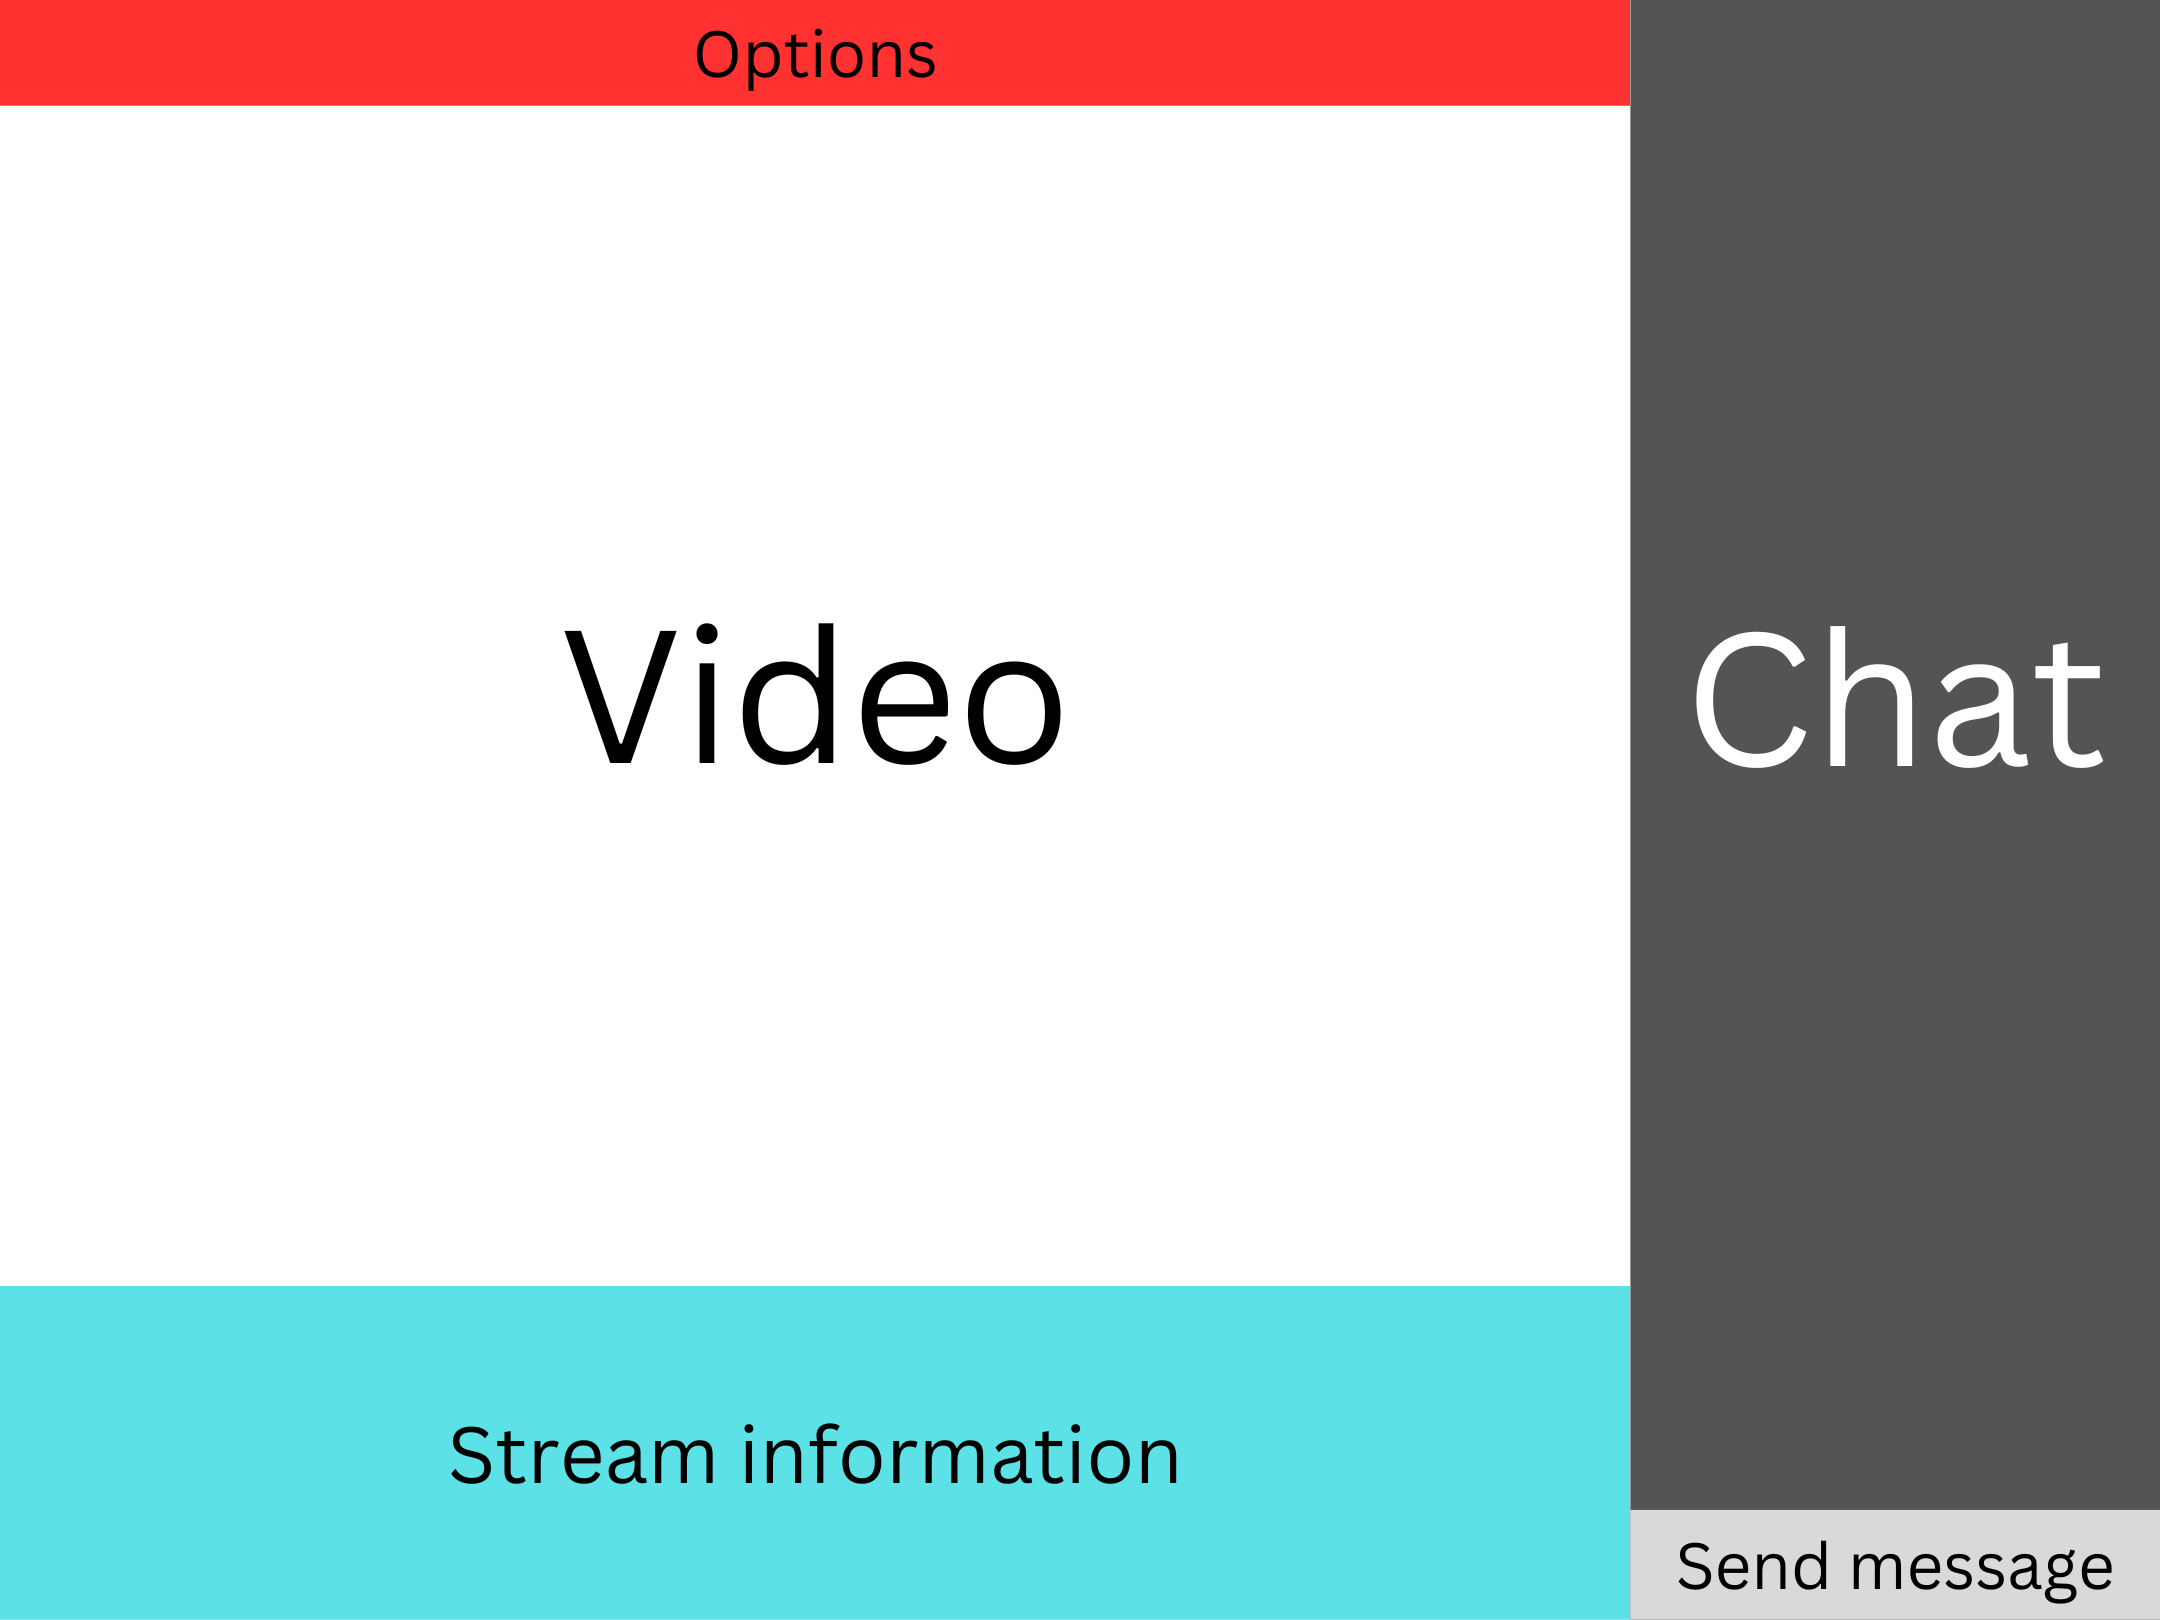
\includegraphics[width=0.8\linewidth]{Chapters/Figures/TwitchStreamSchematic.png}}%
        \caption{Typical structure of \href{https://www.twitch.tv/}{Twitch} video streams, featuring its main elements}
        \label{fig:TwitchStreamStructure}
    \end{figure}

    Within the overall structure, three visual elements play crucial roles in conveying information about the events in a gaming broadcast. The Video element visually showcases the gameplay, while the Chat facilitates viewer interaction with the broadcaster and fellow viewers. Additionally, the stream information element offers details about the content, including the name of the video game being played, the channel name, the stream title, and the relevant categories for the broadcast.

    \subsubsection*{Twitch Engineering}

    The \href{https://www.twitch.tv/}{Twitch} platform has many engineering teams trying to empower live interactive communities, fostering the creation of unique, unforgettable moments in the dynamic interactions between streamers and their audiences. To reach this goal of a consistently high-quality experience in a seemly way these teams create services and tools and these are some of the steps \cite{TwitchEngineering}.

    The Twitch Video Ingest team manages the challenge of handling hundreds of thousands of simultaneous live video streams and distributing them globally. This is achieved through a system where creators' streams are received and prepared for viewing. Twitch operates data centers, referred to as edges, distributed globally and connected to local \gls{ISP}. These edges enable streamers to quickly connect to the network, ensuring optimal video quality. Upon connection, the edge directs the stream to larger data centers known as Origins, which host numerous servers dedicated to transcoding streams into various bitrates and formats for the Twitch \gls{CDN}. This intricate process ensures viewers worldwide, on any network, can seamlessly watch their favorite streams.

    Following video ingestion, the crucial next step is transcoding, where the streamers' video streams undergo conversion into formats conducive to an optimal playback experience. This ensures an excellent viewing experience regardless of the viewer's device capabilities or network conditions.

    The transcoding system takes the incoming \gls{RTMP} stream from the streamer and transforms it into an \gls{HLStream}-compliant stream. This transformative process generates multiple variations of the stream with diverse video resolutions and bitrates, offering viewers the flexibility to watch at the highest possible quality.

    Upon arrival at an Origin and completion of the transcoding process, the responsibility of delivering the stream to viewers swiftly falls under the purview of Video Distribution. \href{https://www.twitch.tv/}{Twitch} upholds a global network of distributed data centers organized in a directed graph hierarchy known as a Replication Tree.

    When a viewer loads a live video page on \href{https://www.twitch.tv/}{Twitch}, their request is intelligently routed to the nearest available data center. From there, the stream request is forwarded up to the Replication Tree. This hierarchical structure ensures an efficient and optimized delivery process. Ultimately, the request reaches the Origin, which promptly returns the stream data to the viewer, facilitating a seamless and quick streaming experience.

    In case not all viewers could watch the stream live the creators can record a \gls{VOD} of their content and distribute it, being from all the stream or some of the best moments. The last one is denominated as Highlights.

